\chapter{Proposta de Trabalho}
\label{chapter:proposta}

\section{Caracterização da pesquisa}

Atualmente, temas relacionados ao ensino e aprendizagem têm sido cada vez mais discutidos e estudados pela comunidade científica. Em especial, ambientes computacionais de aprendizagem têm apresentando uma crescente importância, desempenhando um papel fundamental em atividades de ensino e treinamento, sendo relevantes não apenas no âmbito acadêmico como também no que se refere à inclusão social/digital de pessoas com necessidades especiais no mundo todo \cite{Svetlana2009,Bersch2017}.

Em uma perspectiva relacionada, o advento da tecnologia vem impactando positivamente as dinâmicas de ensino e aprendizagem. Particularmente, a união entre as TICs e práticas pedagógicas modernas tem proporcionado ambientes educacionais mais dinâmicos e inclusivos \cite{Cilli2017}. Nesse contexto, este trabalho tem como principal objetivo propor uma infraestrutura que auxilie na criação de aplicações educacionais inclusivas com apoio a línguas de sinais e educação bilíngue.

Para isso, refletir sobre os estudos primários obtidos no MS deste trabalho foi fundamental. De modo geral, a maioria das soluções identificadas conduziu a fase de desenvolvimento do software sem seguir padrões/técnicas de reuso da ES. Isso resultou em aplicações monolíticas geralmente focadas em um domínio de ensino e aprendizagem específico, prejudicando assim o compartilhamento de seus recursos educacionais e criando soluções acessíveis, mas não inclusivas.

Em contrapartida, algumas contribuições investigam conceitos mais interessantes do ponto de vista técnico, os quais possibilitam o compartilhamento ordenado de recursos educacionais e/ou tecnológicos. Nesse sentido, os seguintes conceitos foram identificados como potenciais abstrações para esta proposta de trabalho:

\begin{itemize}
    \item \textbf{Arquitetura}: pode ser definida como uma estrutura ou organização lógica de componentes, com suas respectivas interações e estrutura da informação \cite{Pressman2016}. %Entretanto, existem inúmeras variações deste termo, as quais podem alterar seu nível de abstração e domínio de aplicação, como por exemplo a Arquitetura de Referência ou Arquitetura Pedagógica;
    \item \textbf{\textit{Framework}}: abstração que une códigos comuns entre vários projetos de software com características similares, provendo configurações e componentes genéricos \cite{Sommerville2015}.
\end{itemize}

Por definição, \textit{frameworks} são menos abstratos que arquiteturas, pois possuem implementações concretas dentro de si. Portanto, entende-se que uma arquitetura seja mais adequada ao contexto deste projeto. Desta forma, as aplicações educacionais poderão ser desenvolvidas com mais liberdade em termos de implementação, desde que a arquitetura proposta seja respeitada. Em particular, optou-se pela Arquitetura Orientada a Serviços (SOA -- \textit{Service-Oriented Architecture}), principalmente pela sua flexibilidade e consonância com as infraestruturas em nuvem atuais.

Por meio de uma arquitetura SOA, é possível construir uma API genérica voltada ao domínio das aplicações educacionais com suporte as línguas de sinais. De fato, APIs são uma das formas mais utilizadas pela indústria para o compartilhamento de recursos, pois elas podem expor interfaces de software totalmente personalizáveis em termos de acesso à informação, permitindo assim integrações seguras e gerenciáveis. Nesse contexto, o estilo arquitetural \textit{\textbf{RE}presentational \textbf{S}tate \textbf{T}ranfer} (REST) merece destaque, principalmente devido a sua total sinergia com o protocolo \textit{HyperText Transfer Protocol} (HTTP) \cite{Fielding2000}, o precursor da Web moderna.

Adicionalmente, o conceito de REA, apesar de identificado em apenas um estudo no MS \cite{BRA23}, é considerado intrínseco nesta proposta, principalmente tendo em vista a criação da API de forma pública e colaborativa para prover recursos de ensino/aprendizagem baseados em línguas de sinais. Com isso, a abstração de software idealizada para este projeto é uma arquitetura SOA baseada no estilo arquitetural REST, a qual será desenvolvida e disponibilizada como um software livre, respeitando as premissas dos REAs. %Entretanto, esta decisão ainda será avaliada, considerando especialistas na área da ES.

De modo geral, o objetivo principal deste projeto de doutorado é prover uma infraestrutura que permita a criação de aplicações educacionais no contexto do ensino bilíngue, de forma simples e padronizada. Para isso, uma API será desenvolvida e implantada para abstrair grande parte da complexidade desse domínio de aplicação. Dessa forma, várias soluções poderão ser instanciadas a partir dessa arquitetura central, as quais poderão explorar os tópicos educacionais pertinentes/permitidos aos seus respectivos contextos.

A título de ilustração, considere o \textit{Hand Talk}, um dos aplicativos de Libras com maior destaque em âmbito nacional. Este aplicativo tem algumas funcionalidades interessantes pensando no desenvolvimento de soluções baseadas na infraestrutura proposta (\autoref{proposal:handtalk}): (i) tradução de texto e áudio para Libras, a qual é interpretada por um avatar 3D. De modo adicional, o usuário também pode optar por mudar a língua de sinais para a ASL; (ii) dicionário categorizado com a representação das palavras em sinais (disponível apenas para a Libras); e (iii) vídeos educacionais  (disponíveis apenas para a Libras) abordando tópicos de interesse dos usuários do aplicativo.

\begin{figure}[htbp]
\centering
\caption{Aplicativo \textit{Hand Talk}}
\label{proposal:handtalk}
\begin{tabular}{ccc}
\frame{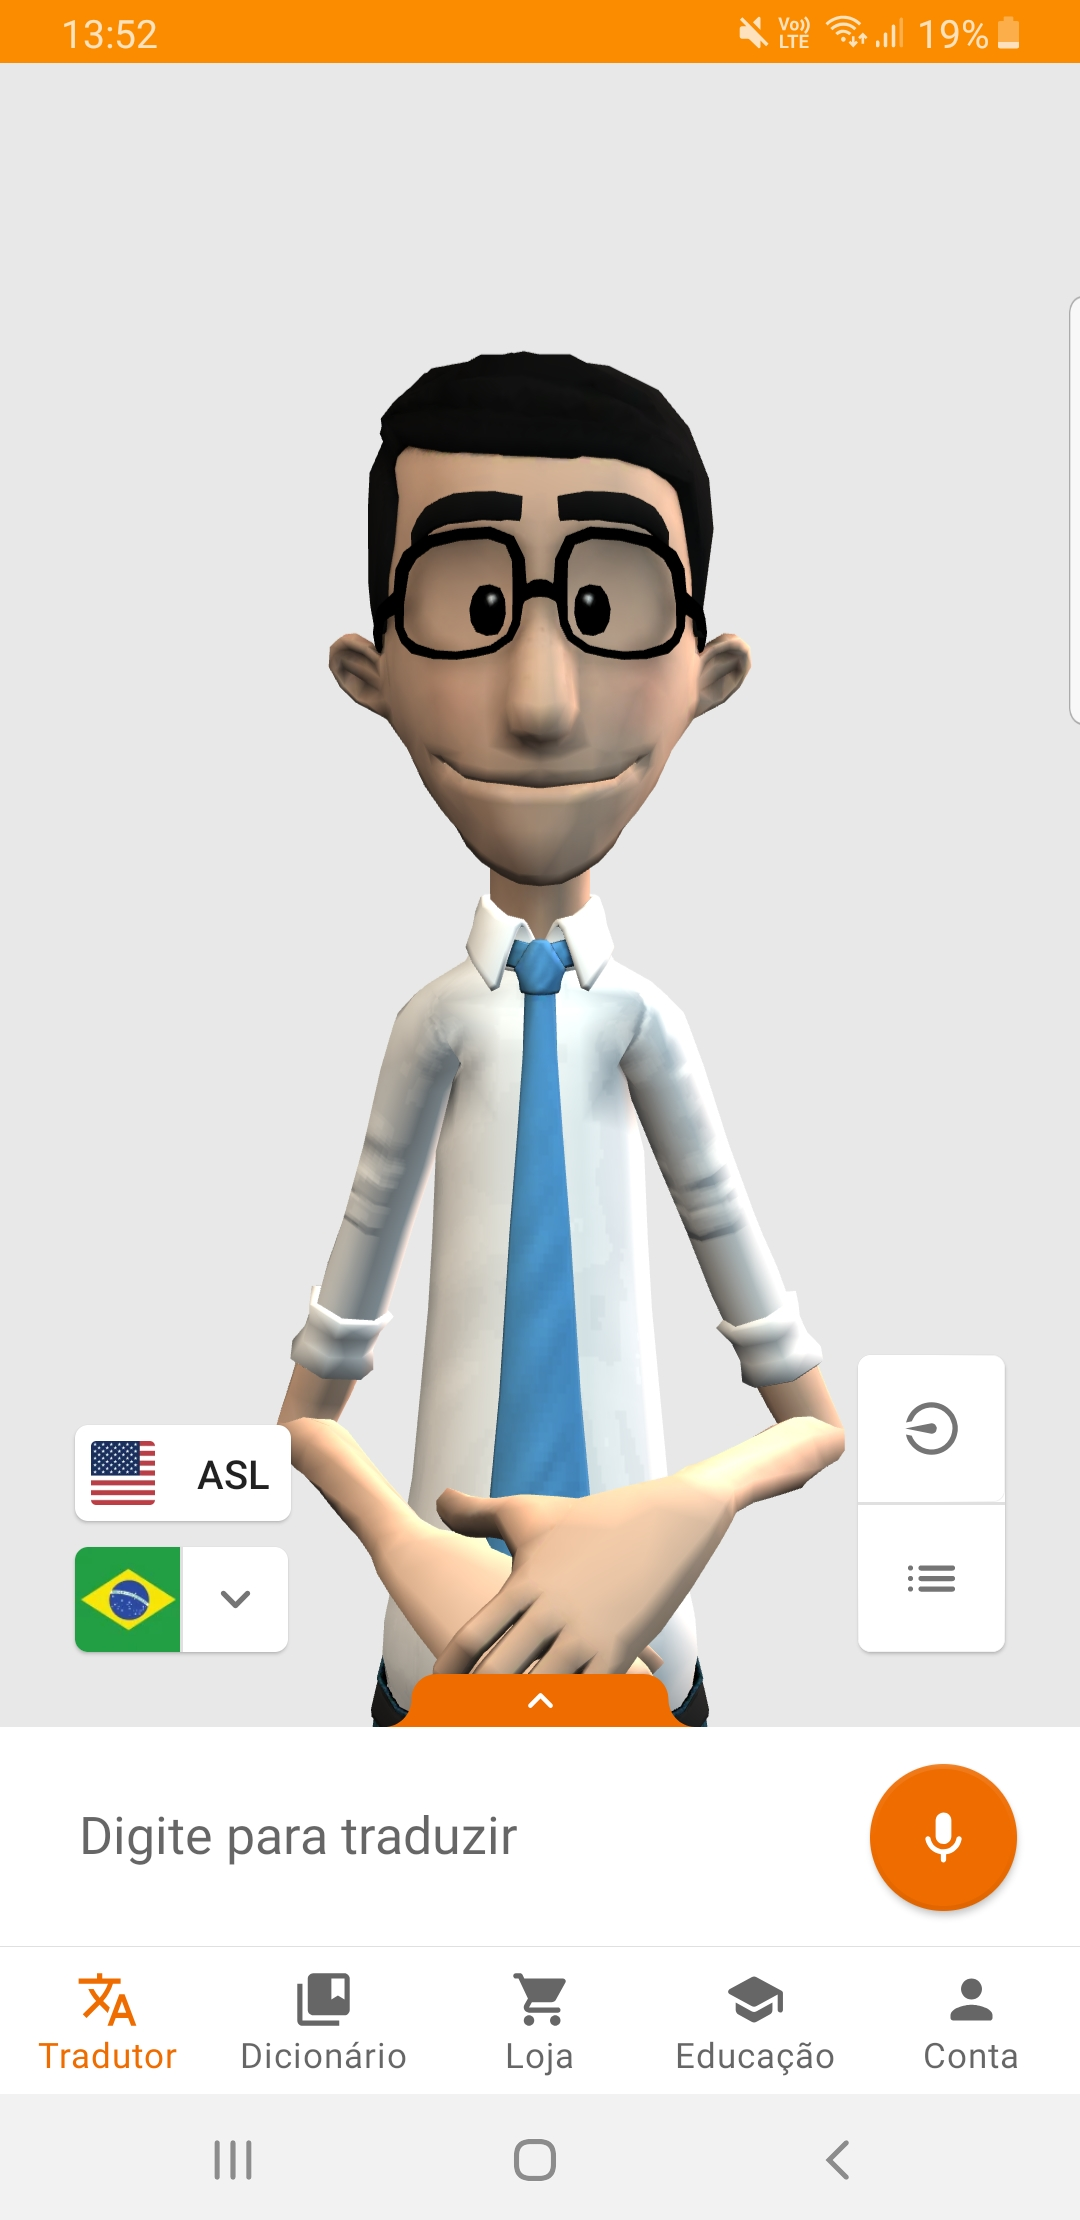
\includegraphics[width=0.3\textwidth]{images/handtalk-01.jpg}} & \frame{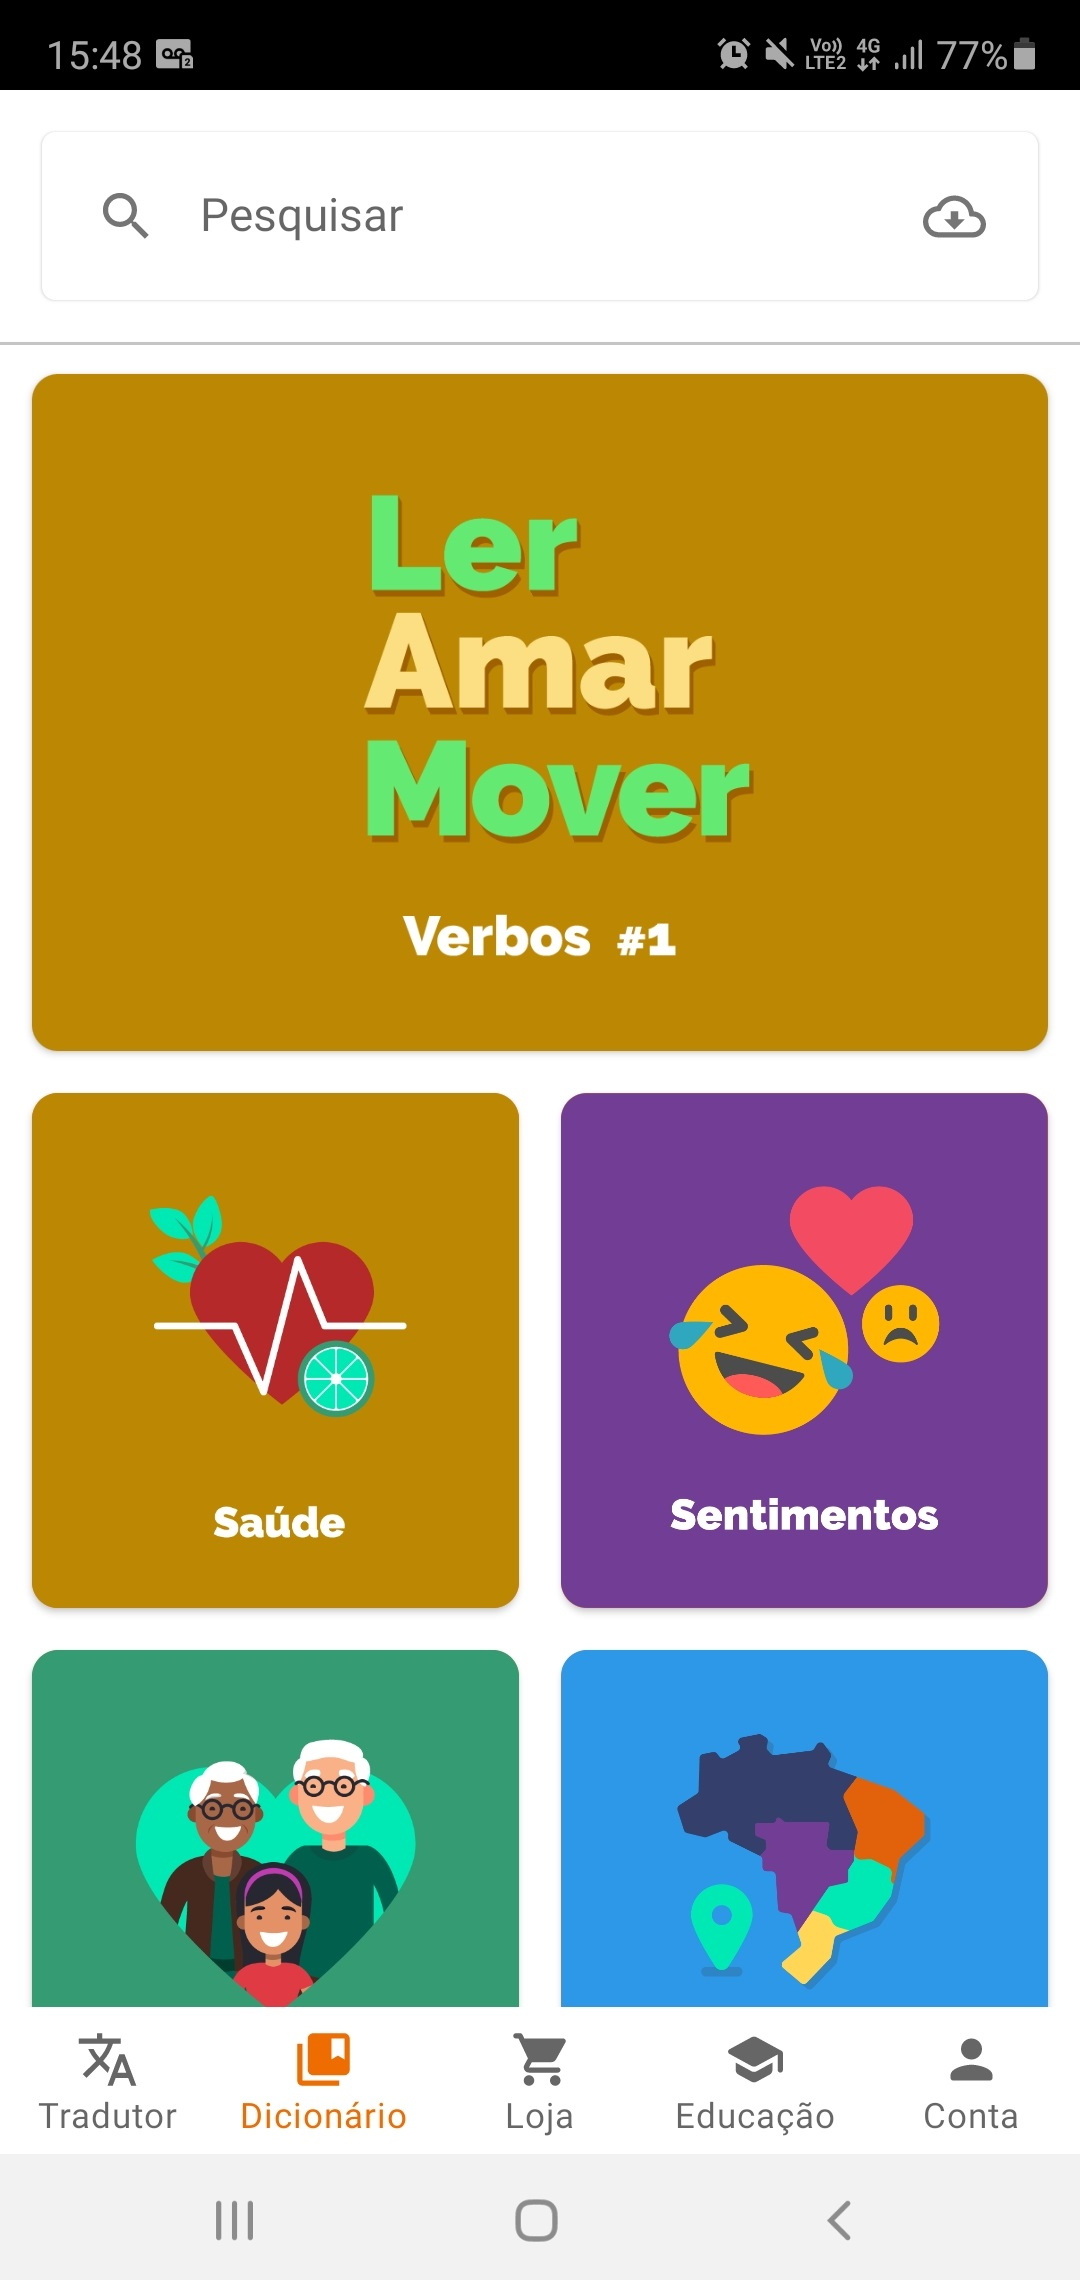
\includegraphics[width=0.3\textwidth]{images/handtalk-02.jpg}} & \frame{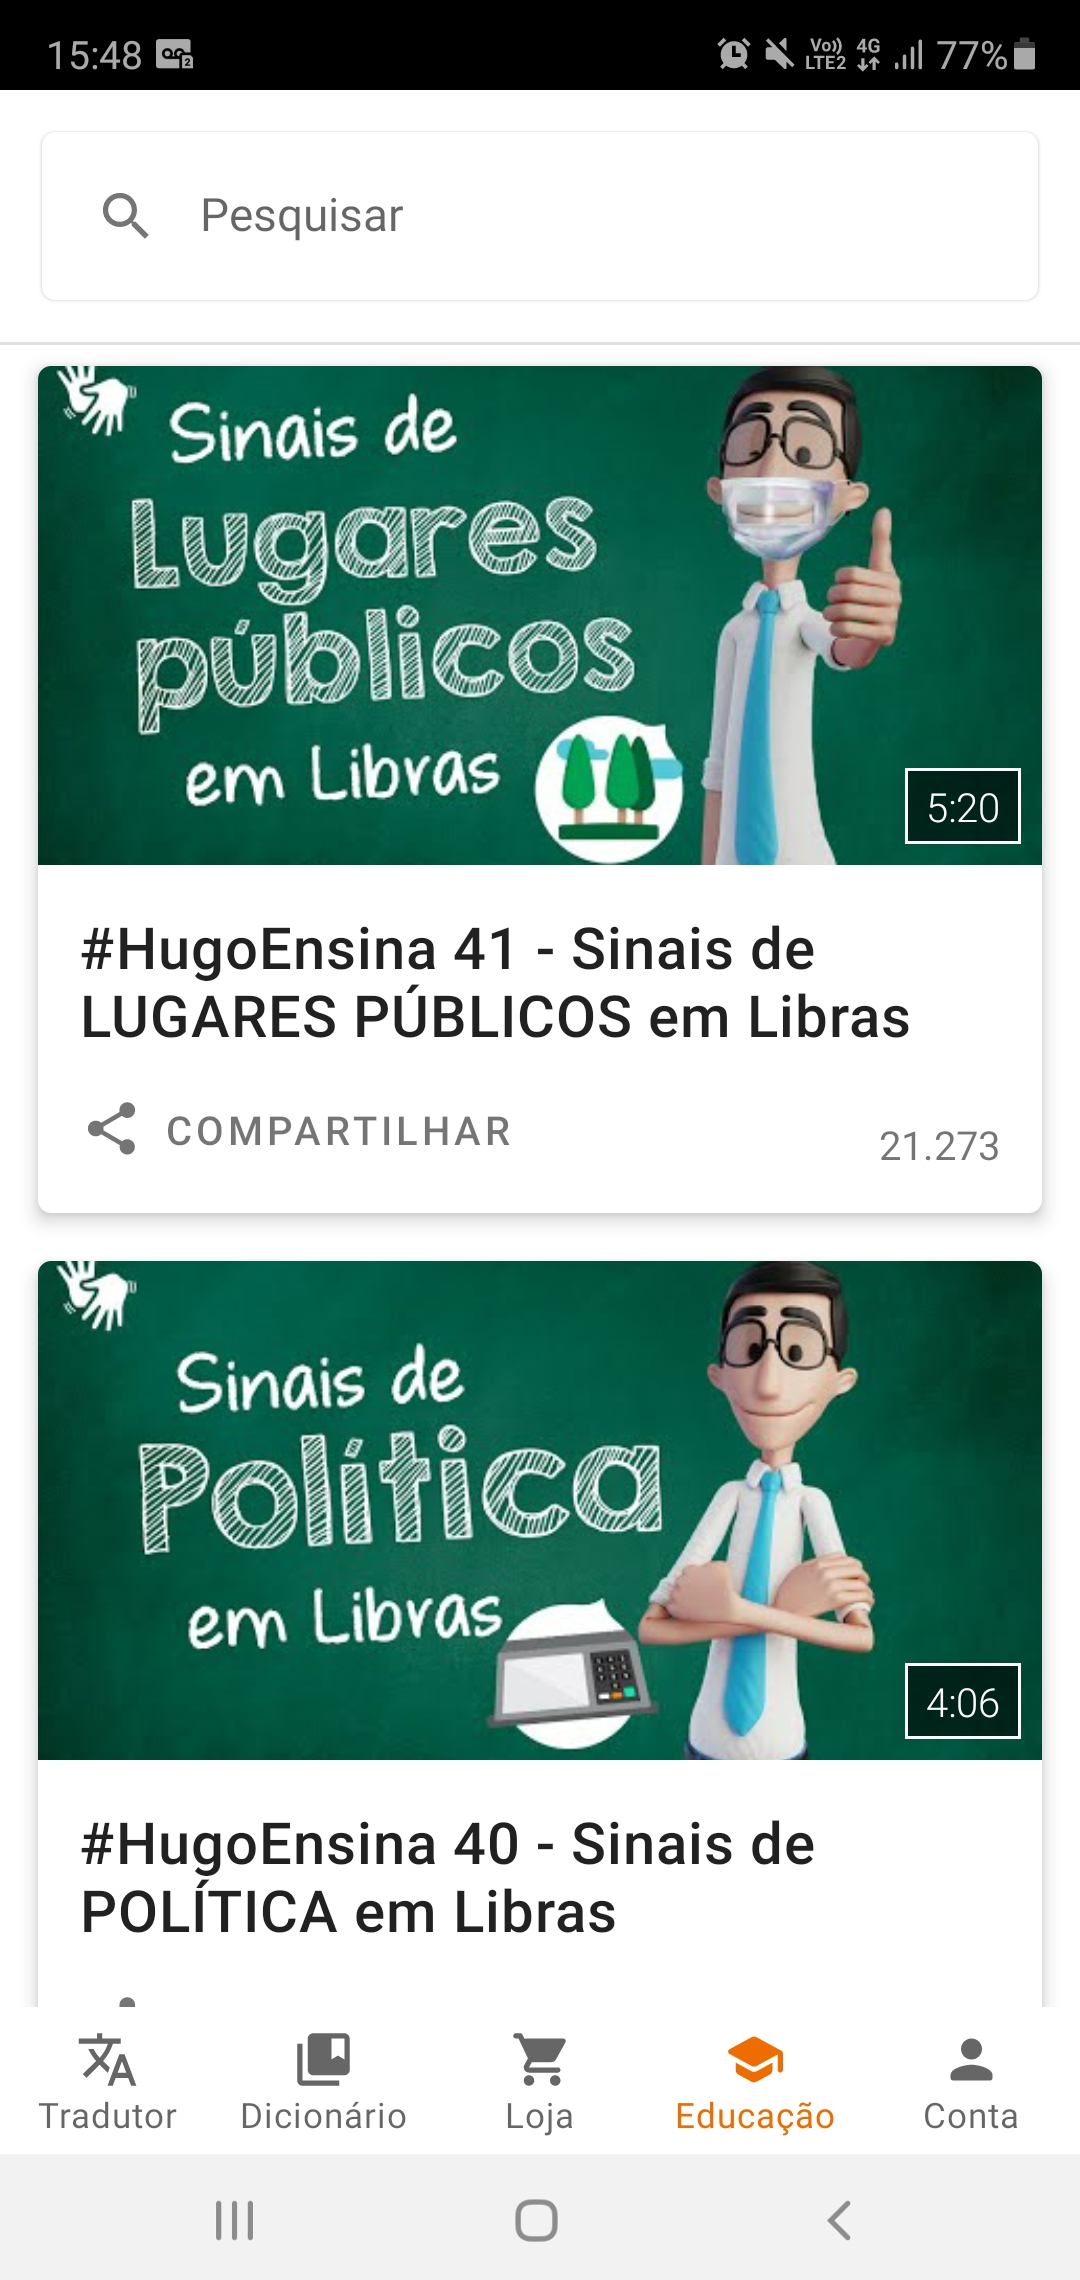
\includegraphics[width=0.3\textwidth]{images/handtalk-03.jpg}}\\
(i) Tradutor & (ii) Dicionário & (iii) Educação \\
\end{tabular}
\caption*{Fonte: \url{www.handtalk.me}.}
\end{figure}

Nesse contexto, entende-se que a gama de soluções no domínio educacional é extensa. Sendo assim, para a criação de uma solução baseada na infraestrutura proposta, optou-se por um tópico de ensino comum e fundamental a ambas línguas (Libras e Português), a Matemática. Consequentemente, uma solução bilíngue é desenhada, com a qual falantes e sinalizantes podem interagir por meio de uma experiência inclusiva. Em termos técnicos, optou-se por uma aplicação educacional móvel, tendo em vista a grande relevância desses dispositivos apresentada nas Seções \ref{chapter:fundamentacao-teorica} e \ref{chapter:mapeamento-sistematico} deste trabalho. Por outro lado, arquiteturalmente, a API é a responsável pela maior parte do esforço computacional da infraestrutura em questão. A seguir, algumas das tarefas de desenvolvimento pretendidas são descritas:  %algumas dessas possibilidades estão sendo analisadas quanto a viabilidade de implementação, são elas:

\begin{itemize}
    \item Tradução de máquina: para que seja possível a tradução bidirecional (texto/voz para língua de sinais e língua de sinais para texto/voz) técnicas de IA devem ser investigadas, principalmente tendo vista algoritmos relacionados à visão computacional (``ler'' os sinais) e redes neurais (tradução);
    \item Internacionalização (I18n) e Localização (L10n): explorando recursos de geolocalização, espera-se que as soluções instanciadas sejam sensíveis ao contexto de seus usuários. Pode-se, com isso, adaptar-se a uma variação regional de uma das línguas, quando necessário. Além disso, essa estrutura pode viabilizar a tradução entre línguas de sinais, possibilitando a comunicação entre uma pessoa fluente em ASL e outra em Libras, por exemplo;
    \item Criação de conteúdo educacional: uma estratégia colaborativa é idealizada, na qual usuários fluentes (muitas vezes professores) criam as atividades em um painel administrativo. Com isso, seus respectivos alunos são notificados sobre esses novos desafios. Consequentemente, uma base de dados extremamente rica é criada, a qual, com o tempo, proverá recursos educacionais cada vez mais efetivos e adequados ao contexto de seus aprendizes. Além disso, como a infraestrutura idealizada é genérica com relação às línguas de sinais, línguas menos evidentes (como as locais e rurais) também podem ser exploradas, mantendo assim seu legado linguístico. %aqui temos uma série de alternativas, dentre as mais interessantes estão a criação de recursos para o ensino de línguas de sinais ou, visando uma validação inicial, o alfabeto. Além disso, o conceito de gamificação se mostrou bastante presente nos estudos primários, indicando uma linha de pesquisa em evidência.
\end{itemize}

\section{Atividades e cronograma}

Tendo em vista os objetivos pretendidos, esta seção define o plano de trabalho e o cronograma idealizados para a condução das tarefas deste projeto de doutorado. Nesse sentido, uma síntese das principais atividades a serem executadas é apresentada a seguir:

\begin{enumerate}
    \item [A.]\textbf{Levantamento e estudo sobre línguas de sinais e TICs na educação:} esta atividade consiste na investigação de referenciais teóricos para identificação dos principais conceitos e limitações relacionados ao ensino e aprendizagem em dois domínios específicos: (i) línguas de sinais; e (ii) TICs. Sendo assim, os temas inclusão digital e educação inclusiva possuem grande relevância para a criação de ambientes de ensino cada vez mais acessíveis em todos os aspectos;
    
    \item [B.]\textbf{Mapeamento Sistemático sobre tecnologia, educação e línguas de sinais:} visa realizar uma busca sistemática e abrangente com a intenção de selecionar estudos relevantes para extração e análise de informações pertinentes às questões de pesquisa estabelecidas. Com isso, espera-se obter uma visão geral sobre o estado da prática com relação ao uso da tecnologia como ferramenta de apoio na educação baseada em línguas de sinais;
    
    \item [C.]\textbf{Proposição de uma arquitetura SOA para a criação de aplicações educacionais baseadas em línguas de sinais:} a partir dos estudos identificados pelas atividades A e B, esta tarefa consiste em projetar a arquitetura em questão para a validação da mesma.%o desenvolvimento de aplicações com arquitetura e recursos educacionais compartilhados. Desta forma, a solução se beneficia exponencialmente do reuso e colaboração de suas instâncias, criando uma base de conhecimento cada vez mais rica e eficiente em resolver seus problemas de negócio;
    
    \item [D.]\textbf{Avaliação da arquitetura por meio de entrevistas e/ou questionários com especialistas:} esta atividade tem como objetivo avaliar a abstração apresentada por meio do \textit{feedback} de especialistas nos domínios da ES, educação e, se possível, línguas de sinais;
    
    \item [E.]\textbf{Refinamento da arquitetura proposta:} a partir das limitações e problemas identificados na atividade anterior, a arquitetura proposta pode ser refinada/evoluída antes de tornar-se um infraestrutura em nuvem. Portanto, quaisquer artefatos e/ou estruturas devem ser devidamente revisados não apenas com viés técnico, mas também nos âmbitos da educação e línguas de sinais;
    
    \item [F.]\textbf{Criação de uma aplicação educacional móvel para o ensino bilíngue:} esta atividade consiste no desenvolvimento de uma solução, tendo em vista a infraestrutura disponível. Proposta de modo a gerar uma aplicação educacional móvel com suporte a multilínguas, explorando os conceitos de internacionalização e localização. Mais especificamente, pretende-se criar uma solução bilíngue, a qual sirva como TA no processo de educação inclusiva;
    
    \item [G.]\textbf{Avaliação da aplicação:} essa atividade tem como objetivo avaliar o produto criado por meio da condução de experimentos seguindo as recomendações da engenharia de software experimental. Nesse sentido, a aplicação educacional móvel será avaliada experimentalmente a partir de sua utilização em ambientes reais de ensino e aprendizagem. Para isso, a princípio existem duas alternativas: (i) comparar os resultados dos participantes com um grupo que não utilizou nenhuma outra solução educacional; ou (ii) comparar com outro software de ensino e aprendizagem baseado em línguas de sinais;
    
\end{enumerate}

Adicionalmente, para que os objetivos pretendidos neste projeto sejam concretizados e as exigências para a obtenção do título de Doutorado em Ciências de Computação e Matemática Computacional sejam cumpridas, também se fazem necessárias as seguintes atividades:

\begin{enumerate}
    \item[H.] Obtenção de créditos em disciplinas de pós-graduação. 
    \item[I.] Exame de proficiência no idioma inglês.
    \item[J.] Escrita e apresentação da monografia para o exame de qualificação.
    \item[K.] Divulgação dos principais resultados da pesquisa em nível nacional e internacional, especialmente por meio de publicação de artigos científicos em periódicos e conferências de qualidade e impacto.
    \item[L.] Redação e defesa da tese de doutorado.
\end{enumerate}

O \autoref{quadro:cronograma} resume o plano de trabalho ao longo dos 48 meses estimados para a obtenção do título de doutor. Nele as atividades planejadas são apresentadas em um cronograma.

\newcommand{\y}{\rule{13pt}{5pt}}
\newcommand{\x}{\hspace*{6pt}}
\setlength{\tabcolsep}{0.3pt}
\begin{quadro}[!ht] \scriptsize
\centering
\caption{Cronograma de atividades.}
\vspace{0.2cm}
\begin{tabular}{|c|c|c|c|c|c|c|c|c|c|c|c|c|c|c|c|c|c|c|c|c|c|c|c|c|}
  \cline{2-25}
  \multicolumn{1}{c|}{} & \multicolumn{6}{c|}{2019} & \multicolumn{6}{c|}{2020}  & \multicolumn{6}{c|}{2021} & \multicolumn{6}{c|}{2022}\\
  \cline{2-25}
  \multicolumn{1}{c|}{\textbf{}} &
  \rotatebox{90}{Jan-Fev\hspace{2pt}} &
  \rotatebox{90}{Mar-Abr\hspace{2pt}} &
  \rotatebox{90}{Mai-Jun\hspace{2pt}} &
  \rotatebox{90}{Jul-Ago\hspace{2pt}} &
  \rotatebox{90}{Set-Out\hspace{2pt}} &
  \rotatebox{90}{Nov-Dez\hspace{2pt}} &
  \rotatebox{90}{Jan-Fev\hspace{2pt}} &
  \rotatebox{90}{Mar-Abr\hspace{2pt}} &
  \rotatebox{90}{Mai-Jun\hspace{2pt}} &
  \rotatebox{90}{Jul-Ago\hspace{2pt}} &
  \rotatebox{90}{Set-Out\hspace{2pt}} &
  \rotatebox{90}{Nov-Dez\hspace{2pt}} &
  \rotatebox{90}{Jan-Fev\hspace{2pt}} &
  \rotatebox{90}{Mar-Abr\hspace{2pt}} &
  \rotatebox{90}{Mai-Jun\hspace{2pt}} &
  \rotatebox{90}{Jul-Ago\hspace{2pt}} &
  \rotatebox{90}{Set-Out\hspace{2pt}} &
  \rotatebox{90}{Nov-Dez\hspace{2pt}} &
  \rotatebox{90}{Jan-Fev\hspace{2pt}} &
  \rotatebox{90}{Mar-Abr\hspace{2pt}} &
  \rotatebox{90}{Mai-Jun\hspace{2pt}} &
  \rotatebox{90}{Jul-Ago\hspace{2pt}} &
  \rotatebox{90}{Set-Out\hspace{2pt}} &
  \rotatebox{90}{Nov-Dez\hspace{2pt}} 
  \\

  \hline
  
  \hspace{2mm}A\hspace{2mm}   
  & \y & \y & \y & \y & \y & \y & \y & \y & \y & \y & \y & \y  & \x & \x & \x & \x & \x  & \x & \x & \x & \x & \x & \x & \x\\
  \hline
  B
   & \y & \y & \y & \y & \y & \y & \y & \y & \y & \y & \x & \x  & \x & \x & \x & \x & \x  & \x & \x & \x & \x & \x & \x & \x\\
  \hline
  C
  & \x & \x & \x & \x & \x & \x & \x & \x & \x & \x & \x & \x  & \y & \y & \y & \x & \x  & \x & \x & \x & \x & \x & \x & \x\\
  \hline
  D
  & \x & \x & \x & \x & \x & \x & \x & \x & \x & \x & \x & \x  & \x & \y & \y & \x & \x  & \x & \x & \x & \x & \x & \x & \x\\
  \hline
  E
  & \x & \x & \x & \x & \x & \x & \x & \x & \x & \x & \x & \x  & \x & \x & \y & \y & \x  & \x & \x & \x & \x & \x & \x & \x\\
  \hline
  F
  & \x & \x & \x & \x & \x & \x & \x & \x & \x & \x & \x & \x  & \x & \x & \y & \y & \y  & \y & \y & \y & \y & \x & \x & \x\\
  \hline
  G
  & \x & \x & \x & \x & \x & \x & \x & \x & \x & \x & \x & \x  & \x & \x & \x & \x & \x  & \x & \x & \x & \y & \y & \y & \x\\
  \hline
  H
  & \y & \x & \x & \x & \x & \x & \x & \x & \x & \x & \x & \x  & \x & \x & \x & \x & \x  & \x & \x & \x & \x & \x & \x & \x\\
  \hline
  I
  & \y & \x & \x & \x & \x & \x & \x & \x & \x & \x & \x & \x  & \x & \x & \x & \x & \x  & \x & \x & \x & \x & \x & \x & \x\\
  \hline
  J
  & \x & \x & \x & \x & \x & \x & \y & \y & \y & \y & \y & \y  & \x & \x & \x & \x & \x  & \x & \x & \x & \x & \x & \x & \x\\
  \hline
  K
  & \x & \x & \y & \y & \y & \y & \y & \y & \y & \y & \y & \y  & \y & \y & \y & \y & \y  & \y & \y & \y & \x & \x & \x & \x\\
  \hline
  L
  & \x & \x & \x & \x & \x & \x & \x & \x & \x & \x & \x & \x  & \x & \x & \y & \y & \y  & \y & \y & \y & \y & \y & \y & \y\\
  \hline

\end{tabular}
\label{quadro:cronograma}
\normalsize
\fautor
\end{quadro}

Como atividade obrigatória do Programa de Pós-Graduação em Ciência da Computação e Matemática Computacional do ICMC-USP, está a realização das disciplinas e o cumprimento de créditos. Desse modo, a \autoref{proposal:quadro:student-record} apresenta as disciplinas cursadas pelo aluno, bem como carga horária, créditos, frequências, conceitos etc. Cabe ressaltar que o aluno cursou tais disciplinas em regime especial e, sendo assim, sua inscrição como aluno regular teve início em 2019.

\begin{quadro}[htbp]
\def\arraystretch{1.5}
\setlength\tabcolsep{0.1cm}
\centering\scriptsize
\caption{Ficha do aluno, adaptada do Janus}
\label{proposal:quadro:student-record}
\begin{tabular}{|l|m{4.4cm}|c|c|C{1.1cm}|c|c|c|c|c|}
\hline
\multicolumn{1}{|c|}{\textbf{Sigla}} & \multicolumn{1}{c|}{\textbf{Nome da Disciplina}} & \textbf{Início} & \textbf{Término} & \textbf{Carga Horária} & \textbf{Cred.} & \textbf{Freq.} & \textbf{Conc.} & \textbf{Exc.} & \textbf{Situação} \\ \hline
SSC5944-1/1 & Arquitetura de Software & 10/03/16 & 09/05/16 & 90 & 6 & 88 & A & N & Concluída \\ \hline
SCC5900-3/1 & Projeto de Algoritmos & 11/03/16 & 01/07/16 & 180 & 12 & 100 & A & N & Concluída \\ \hline
SCC5912-3/1 & Interação Usuário-Computador I: Fundamentos & 09/08/16 & 04/10/16 & 120 & 8 & 95 & A & N & Concluída \\ \hline
SCC5951-1/1 & Interação Usuário-Computador II: Prática & 11/10/16 & 22/11/16 & 60 & 4 & 100 & A & N & Concluída \\ \hline
SCC5774-4/2 & Inteligência Artificial I & 17/03/17 & 05/05/17 & 90 & 6 & 100 & A & N & Concluída \\ \hline
SSC5916-5/1 & Tópicos em Computação e Matemática Computacional I & 22/03/17 & 05/07/17 & 15 & 1 & 100 & B & N & Concluída \\ \hline
SCC5949-1/2 & Inteligência Artificial II & 12/05/17 & 07/07/17 & 90 & 6 & 100 & A & N & Concluída \\ \hline
SME5919-4/2 & Tópicos Especiais em Computação e Matemática Computacional II & 09/08/17 & 06/12/17 & 15 & 1 & 100 & A & N & Concluída \\ \hline
SCC5933-4/10 & Metodologia de Pesquisa Científica em Computação & 11/08/17 & 06/10/17 & 30 & 2 & 100 & A & N & Concluída \\ \hline
\end{tabular}
\end{quadro}

\begin{quadro}[htbp]
\def\arraystretch{1.5}
\setlength\tabcolsep{0.1cm}
\centering\scriptsize
\begin{tabular}{|l|c|c|c|}
\hline
 & \multicolumn{2}{c|}{\textbf{Créditos mínimos exigidos}} & \textbf{Créditos obtidos} \\ \hline
 & \textbf{Para exame de qualificação} & \textbf{Para depósito de tese} & \textbf{} \\ \hline
\textbf{Disciplinas:} & 0 & 42 & 46 \\ \hline
%\textbf{Estágios:} &  &  &  \\ \hline
\textbf{Total:} & 0 & 42 & 46 \\ \hline
\end{tabular}
\fautor
\end{quadro}

\section{Procedimentos metodológicos}

A partir do problema de pesquisa identificado e os objetivos estabelecidos, buscou-se determinar uma sequência de procedimentos metodológicos, visando a conclusão deste trabalho de doutorado. Os procedimentos metodológicos foram divididos em três blocos, em destaque na \autoref{proposal:figure:objectives-methods-results}: (i) Requisitos; (ii) Projeto e Implementação; e (iii) Avaliação Experimental.

A etapa de \textbf{Requisitos} visa esclarecer lacunas para a continuidade da pesquisa, a qual é composta por: revisão bibliográfica e mapeamento sistemático. A revisão bibliográfica foi conduzida com base em livros, artigos científicos, relatórios estatísticos e aporte legal \cite{Gil2016} e buscou fornecer base teórica sobre conceitos relacionados às línguas de sinais e TICs, auxiliando no \textit{Objetivo 1}. Em seguida um MS foi conduzido respeitando as diretrizes de busca sistemática baseada em QGS estabelecidas por \citeonline{Zhang2011}.

O MS teve como base três QP que buscaram atender aos \textit{Objetivos 2}, \textit{3} e \textit{4}. Sendo assim, esse estudo aferiu a existência de contribuições com potencial de (i) identificar os tipos de soluções investigadas; (ii) classificar os tópicos educacionais mais relevantes; e (iii) apresentar as línguas de sinais mais exploradas. Os resultados desse MS geraram três publicações: a primeira com foco nos resultados internacionais, obtidos através da abordagem baseada em QGS \cite{FalvoJr2020_FIE}, a segunda com foco na busca manual nacional, a qual estendeu nossas discussões sobre a Libras \cite{FalvoJr2020_SBIE} e, por fim, uma discussão estendida sobre os cenários nacional e internacional \cite{FalvoJr2020_RENOTE}.

Mediante a análise dos estudos primários do MS identificou-se que as aplicações educacionais com apoio a línguas de sinais: (i) são frequentemente desenvolvidas de modo \textit{ad hoc}, ocasionando uma diversificação demasiada de técnicas e tecnologias de desenvolvimento, as quais geralmente focam em acessibilidade, mas não em inclusão; (ii) utilizam diferentes estratégias e tópicos de ensino e (iii) em sua maioria, não apresentam possibilidade de compartilhamento de seus recursos educacionais ou tecnológicos. 

Portanto, opta-se pela definição de uma arquitetura SOA para a criação de aplicações educacionais padronizadas no domínio das línguas de sinais, com ênfase na educação inclusiva. Com isso, inicia-se a etapa de \textbf{Projeto e Implementação}, tida como a mais importante deste estudo, a qual contempla a proposição e avaliação da arquitetura (\textit{Objetivo 5}), bem como o desenvolvimento de um produto para o ensino e aprendizagem no contexto bilíngue (\textit{Objetivo 6}).

Finalmente, na etapa \textbf{Avaliação Experimental}, métodos difundidos para a condução de avaliações experimentais na ES, tais como os apresentados por \citeonline{Wohlin2012}, serão considerados para avaliar a instância gerada a partir da arquitetura/infraestrutura proposta (\textit{Objetivo 7}). Vale salientar que as avaliações conduzidas pelos \textit{Objetivos 5} e \textit{7} terão estratégias diferentes, a primeira será feita por especialistas nas áreas de ES, educação e línguas de sinais, visando refinamentos/melhorias na abstração proposta. Por outro lado, a avaliação experimental tende a ser mais formal e, nesse caso, terá foco na qualidade e funcionalidade das instâncias.

\section{Resultados esperados}

Como principais resultados esperados a partir da condução das atividades estabelecidas neste plano de trabalho, destacam-se:

\begin{itemize}
  \item Identificação de um conjunto básico de especificações técnicas, características e requisitos de desenvolvimento relacionados à educação inclusiva baseada em línguas de sinais apoiada pelas TICs;
  
  \item Identificação do estado da prática de soluções educacionais com suporte a língua de sinais mediante o uso de tecnologia, tendo como premissa a condução de um MS para a identificação e análise dos estudos primários;
  
  \item Proposição de uma arquitetura SOA para criação de um arcabouço formal que apoie o desenvolvimento de aplicações educacionais baseadas em línguas de sinais. %Como contribuição secundária, espera-se esclarecer o entendimento a respeito de abordagens ambíguas e recorrentemente mal interpretadas na ES, como as seguintes: Arquitetura, Arquitetura de Referência, Framework, Modelo, Metamodelo etc. Para isso, a condução de um relatório técnico deve ser priorizada; 
  
  \item Avaliação com especialistas da arquitetura proposta, tendo em vista o refinamento e evolução da abordagem em função de \textit{feedbacks} das áreas de ES, educação e línguas de sinais;
  
  \item Desenvolvimento de uma aplicação educacional móvel que instancie a arquitetura proposta com ênfase na educação bilíngue. Além disso, é importante ressaltar que as aplicações geradas a partir dessa infraestrutura comum serão sensíveis ao contexto de seus usuários, explorando os conceitos de internacionalização (i18n) e localização (l10n). Com isso, as aplicações educacionais desenvolvidas terão a capacidade de se adequar à variações regionais de seus usuários;
  
  \item Condução de experimentos com aprendizes e tutores, a fim de avaliar estatisticamente a aplicação educacional supracitada e, indiretamente, sua respectiva base de construção;
  
  \item Elaboração de artigos a serem submetidos a congressos e periódicos da área, tanto em nível nacional como internacional.
\end{itemize}

A \autoref{proposal:figure:objectives-methods-results} sintetiza a relação entre objetivos, procedimentos metodológicos/atividades e resultados esperados.

\begin{sidewaysfigure}[htbp]
\caption{Objetivos, procedimentos metodológicos/atividades e resultados esperados.}
\label{proposal:figure:objectives-methods-results}
\centerline{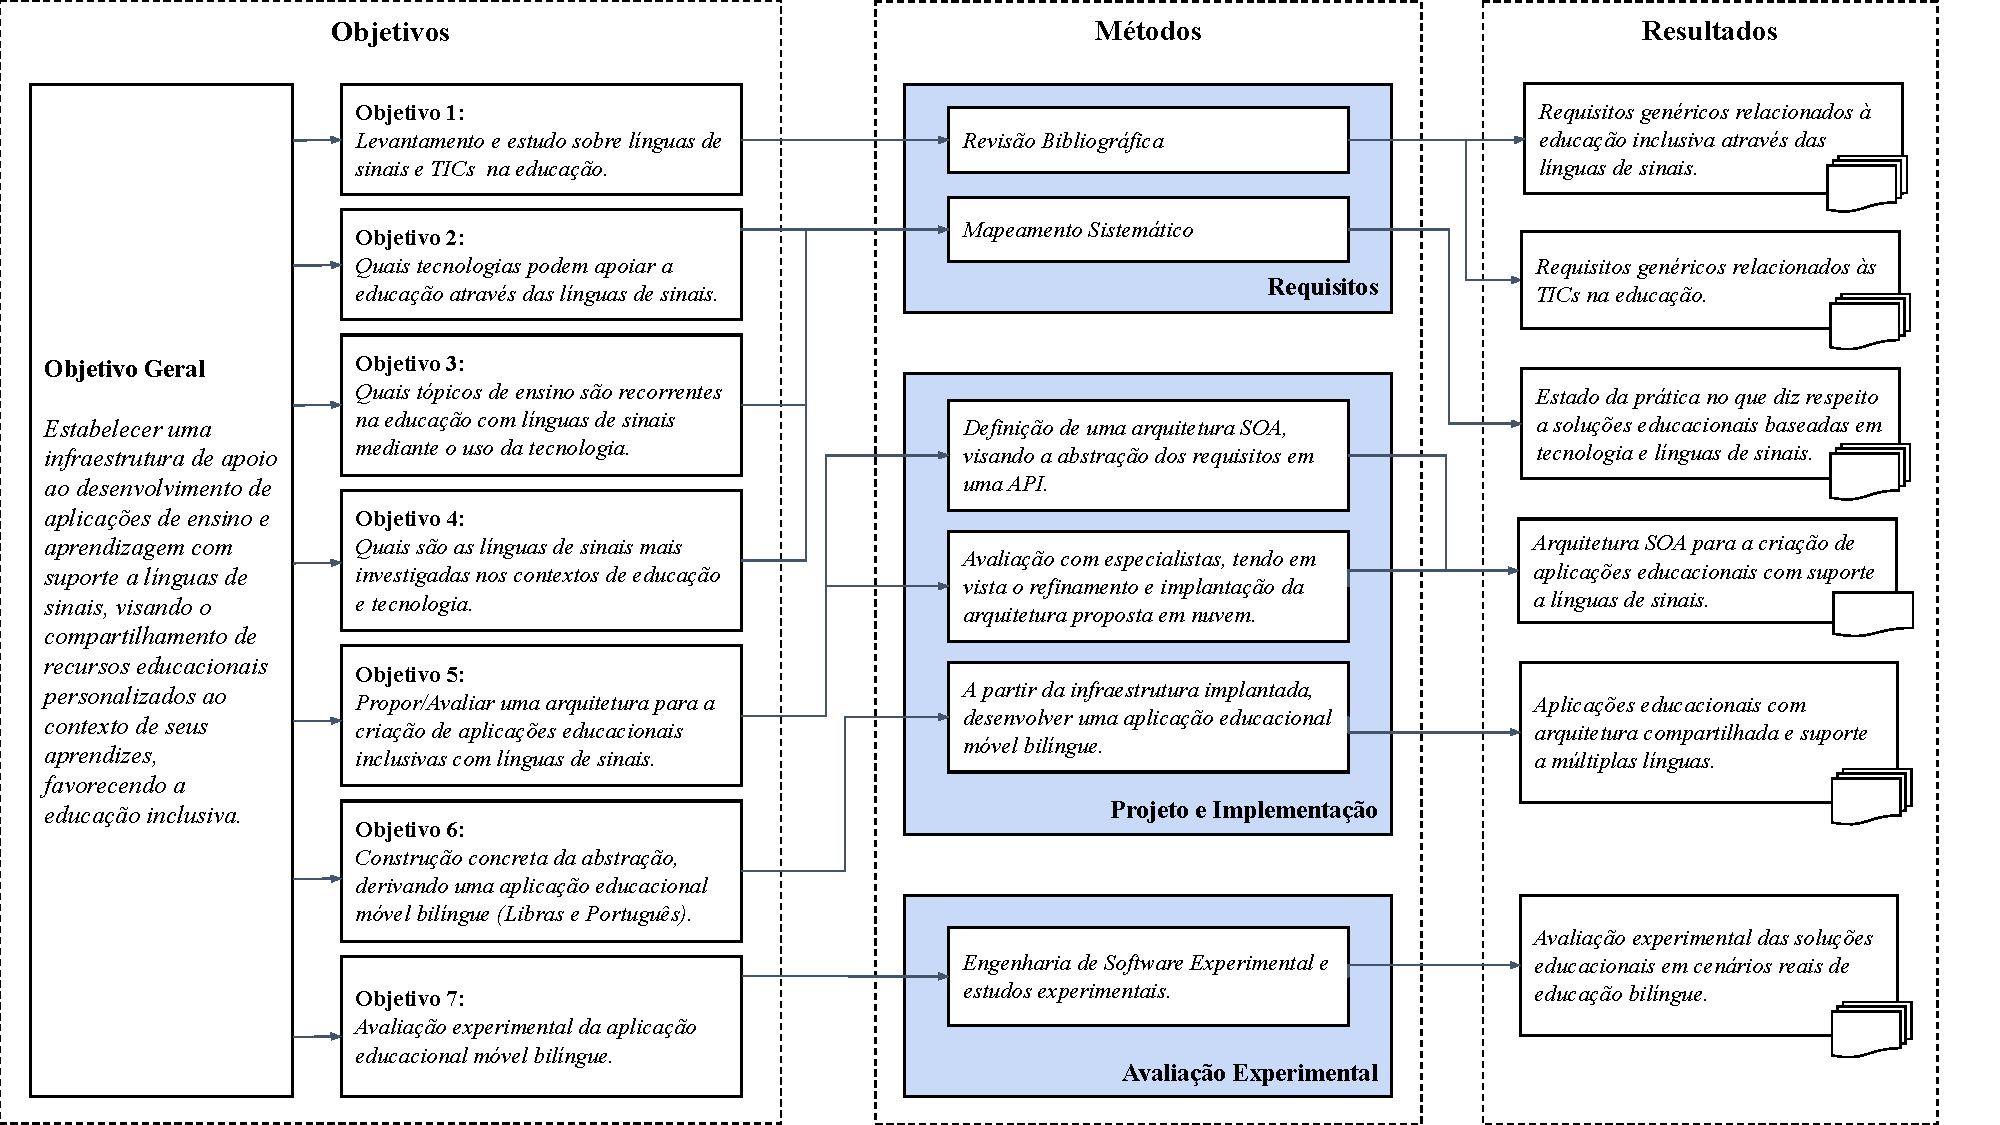
\includegraphics[width=\textwidth]{images/objectives-methods-results.pdf}}
\fautor
\end{sidewaysfigure}

\section{Publicações}

Nesta seção são apresentadas as publicações realizadas no decorrer dos quatro primeiros semestres do doutorando. Algumas delas estão relacionadas a pesquisas conduzidas previamente \cite{Soad2017_FIE, Oliveira2019_SBIE, FalvoJr2020_JUCS}. Entretanto, tais estudos são importantes pois têm relação com as temáticas de ensino e aprendizagem, as quais serão investigadas diretamente neste projeto de doutorado.

\begin{itemize}

\item \uppercase{FalvoJr, V.; Martins Falvo, C.; Scatalon, L. P.; and Barbosa, E. F.} \textit{Tecnologias Aplicadas ao Ensino e Aprendizagem com Línguas de Sinais: Um Mapeamento Sistematico Sob as Perspectivas Nacional e Internacional}. Revista Novas Tecnologias na Educação (RENOTE). 2020. p. 1--13. \textit{Artigo aceito em 09 de Dezembro de 2020}.

\item \uppercase{FalvoJr, V.; Martins Falvo, C.; Scatalon, L. P.; and Barbosa, E. F.} \textit{Tecnologias Aplicadas ao Ensino e Aprendizagem de Libras: Um Mapeamento Sistemático}. Anais do Simpósio Brasileiro de Informática na Educação (SBIE 2020). Natal, RN, Brasil. 2020. p. 1--10. \textit{Artigo apresentado remotamente pelo autor principal}.

\item \uppercase{FalvoJr, V.; Scatalon, L. P.; and Barbosa, E. F.} \textit{The Role of Technology to Teaching and Learning Sign Languages: A Systematic Mapping}. Proceedings of the 50th Annual Frontiers in Education Conference (FIE 2020). Uppsala, Suécia. 2020. p. 1--10. \textit{Artigo apresentado remotamente pelo autor principal}.

\item \uppercase{FalvoJr, V.; Marcolino, A. S.; Duarte Filho, N. F.; OliveiraJr, E. A.; Barbosa, E. F.} \textit{Variability-based improvement of m-learning applications development}. Journal of Universal Computer Science (J.UCS). 2020. p. 1--25. \textit{Artigo em processo de avaliação, submetido em 04 de Fevereiro de 2020}.

\item \uppercase{Oliveira, R.; FalvoJr, V.; Barbosa, E. F.} \textit{Internet das Coisas aplicada à Educação: Um Mapeamento Sistemático}. Anais do Simpósio Brasileiro de Informática na Educação (SBIE 2019). Brasília, DF, Brasil. 2019. p. 499--508. \textit{Artigo apresentado presencialmente pelo autor principal}.

\item \uppercase{Soad, G. W.; Fioravanti, M. L.; FalvoJr, V.; Marcolino, A.; Duarte Filho, N. F.; Barbosa, E. F.} \textit{ReqML-catalog: The road to a requirements catalog for mobile learning applications}. Proceedings of the 47th Annual Frontiers in Education Conference (FIE 2017). Indianapolis, IN, USA. 2017. p. 1–9. \textit{Artigo apresentado presencialmente pelo autor principal}.

\end{itemize}